\documentclass[letterpaper,12pt]{article}
% \usepackage[utf8]{inputenc}
\usepackage{graphicx}
\usepackage{ifpdf}

% \usepackage[spanish,mexico]{babel}
\usepackage{multicol}
\usepackage{tikz}

\usepackage{amssymb}
\usepackage{amsmath}


%opening
\title{Lecture 2}
\author{Isaac Ayala Lozano}

\begin{document}

% \maketitle



\section{Lecture 2 - Exercise 8}

Calculate the velocity, speed and acceleration for each 
position vector.


% --------------------------

\subsection{$\vec{r}(t)= (\cos (\omega t), \mathrm{e}^{\omega t})$}

The first derivative of the vector gives us

\begin{equation*}
 \vec{v}(t) = (- \omega \sin (\omega t), \omega \mathrm{e}^{\omega t})
 \end{equation*}

The norm of the velocity vector gives us the speed.
 
 \begin{equation*}
  \left \| \vec{v}(t) \right \| = \sqrt{ \omega^2 \sin^2 (\omega t) + \omega ^2 
\mathrm{e}^{2 \omega t}}
 \end{equation*}

 The second derivative results in 
 
 \begin{equation*}
  \vec{a}(t) = (-\omega ^2 \cos (\omega t) , \omega ^2 
\mathrm{e}^{\omega t})
 \end{equation*}

Figure \ref{fig: vector 1} shows the plots for all three vectors with 
conditions $\omega = 1$, and $t \in \left [ 0, 2 \pi \right ] $.
 
\begin{figure}[h]
 \centering

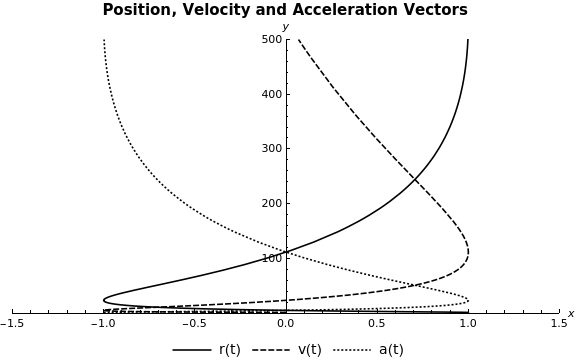
\includegraphics[scale=0.65,keepaspectratio=true]{./img/graph01.png}
 \caption{Position, Velocity and Acceleration plots for 
$\vec{r}(t)= (\cos (\omega t), \mathrm{e}^{\omega t})$
}
 \label{fig: vector 1}
\end{figure}


% -----------------------

\subsection{$\vec{r}(t) = ( \cos (\omega t - \phi), \sin (\omega t - \phi))$}

Using the following trigonometric identities

\begin{equation*}
 \begin{split}
  \sin (\alpha \pm \beta) & = \sin \alpha \cos \beta \pm \cos \alpha \sin \beta 
\\
\cos (\alpha \pm \beta & = \cos \alpha \cos \beta \mp \sin \alpha \sin \beta
 \end{split}
\end{equation*}

the position vector can be rewritten as follows

\begin{equation*}
 \vec{r} = (
 \cos \omega t \cos \phi + \sin \omega t \sin \phi,
 \sin \omega t \cos \phi - \cos \omega t \sin \phi
 )
\end{equation*}

The velocity, speed and acceleration are as follows

 \begin{equation*}
 \begin{split}
 \vec{v}(t) & = ( - \omega \cos \phi \sin \omega t + \omega \sin \phi \cos 
\omega t, \omega \cos \phi \cos \omega t + \omega \sin \phi \sin \omega t) \\
& = (- \omega \sin (\omega t + \phi), \omega \cos (\omega t + \phi))
 \end{split}
 \end{equation*}


\begin{equation*}
 \left \| \vec{v}(t) \right \| = \sqrt{ \omega ^2 \sin ^2 (\omega t + \phi) + 
\omega ^ 2 \cos ^2 (\omega t + \phi)}
\end{equation*}

 \begin{equation*}
 \begin{split}
  \vec{a}(t) & =  ( - \omega ^2 \cos \phi \cos \omega t - \omega ^2 \sin \phi 
\sin \omega t, - \omega ^2 \cos \phi \sin \omega t + \omega ^2 \sin \phi \cos 
\omega t)\\
& = ( - \omega ^2 \cos (\omega t - \phi), -\omega ^ 2 \sin (\omega t - \phi))
 \end{split}
 \end{equation*}
 
 Figure \ref{fig: vector 2} shows the plotted movement equations for the 
system. Notice that all three curves overlap when evaluated with $\omega = 1$, 
 $t \in \left [ 0, 2 \pi \right ] $ and $\phi = \frac{\pi}{4}$.
 
 \begin{figure}[h]
 \centering
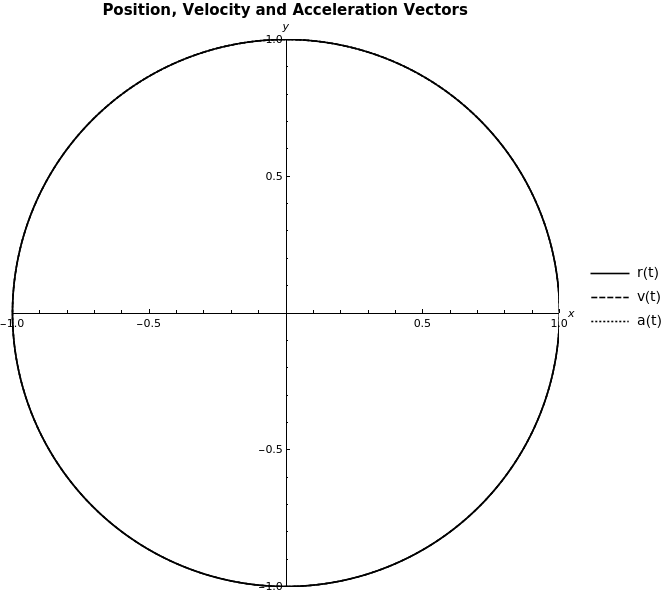
\includegraphics[scale=0.4,keepaspectratio=true]{./img/graph02.png}
 \caption{Position, Velocity and Acceleration plots for 
$\vec{r}(t) = ( \cos (\omega t - \phi), \sin (\omega t - \phi))$
}
 \label{fig: vector 2}
\end{figure}


% ----------------------


\subsection{$\vec{r}(t) = ( c \cos ^3 (t), c \sin ^3 (t))$}

Apply the chain rule to obtain the derivatives of $\vec{r}(t)$.

 \begin{equation*}
  \vec{v}(t) = (- 3 c \cos ^2 (t) \sin (t), 3 c \sin ^ 2 (t) \cos (t))
 \end{equation*}


\begin{equation*}
 \left \| \vec{v}(t) \right \| = \sqrt{ 9 c^2 \cos ^4 (t) \sin^2 (t) + 9 c^2 
\sin ^4 (t) \cos ^2 (t)}
\end{equation*}

 \begin{equation*}
  \vec{a}(t) = (- 3 c \cos ^3 (t) - 6 c \sin ^2 (t) \cos (t), -3 c \sin ^3 (t) 
+ 6 c \cos ^2 (t) \sin (t))
 \end{equation*}
 
 All three vectors are plotted in figure \ref{fig: vector 3} with $t \in 
\left [ 0, 2 \pi \right ] $, and $c = 1$.
 
 \begin{figure}[h]
 \centering

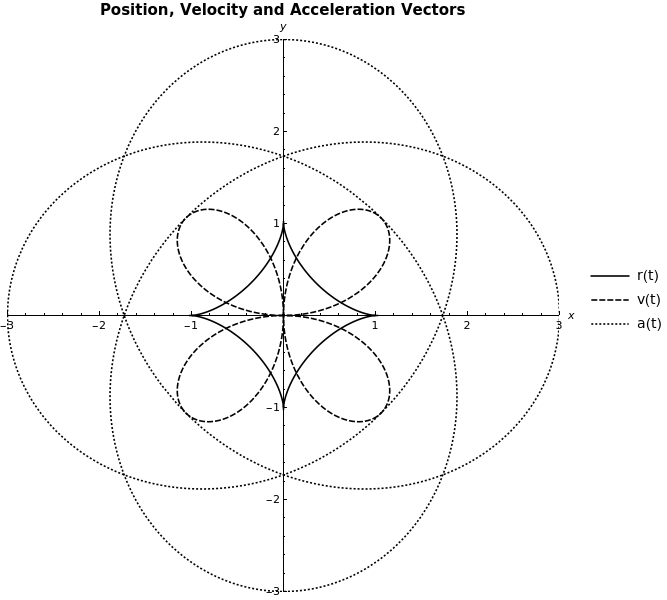
\includegraphics[scale=0.4,keepaspectratio=true]{./img/graph03.png}
 \caption{Position, Velocity and Acceleration plots for 
$\vec{r}(t) = ( c \cos ^3 (t), and c \sin ^3 (t))$.
}
 \label{fig: vector 3}
\end{figure}


% ---------------------------


\subsection{$\vec{r}(t) = ( c (t - \sin t), c (1 - \cos t))$}
 
  \begin{equation*}
  \vec{v}(t) = (c (1 - \cos (t) ), c \sin (t))
 \end{equation*}


\begin{equation*}
 \left \| \vec{v}(t) \right \| = \sqrt{ c^2 - c^2 \cos ^2 (t) + c^2 \sin ^2 (t)}
\end{equation*}

 \begin{equation*}
  \vec{a}(t) = (c \sin (t), c \cos (t))
 \end{equation*}
 
 Figure \ref{fig: vector 4} shows the plots for all three equations evaluated 
with $c = 1$ and $t \in 
\left [ 0, 2 \pi \right ] $.
 
 \begin{figure}[h]
 \centering

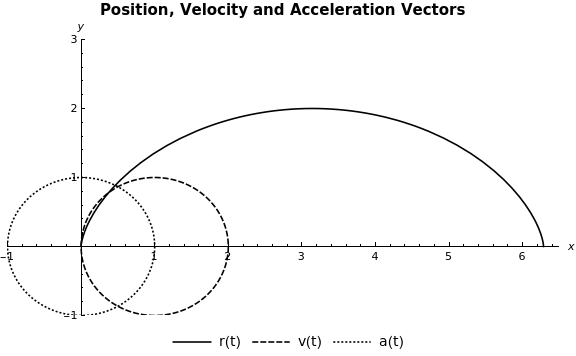
\includegraphics[scale=0.4,keepaspectratio=true]{./img/graph04.png}
 \caption{Position, Velocity and Acceleration plots for 
$\vec{r}(t) = ( c (t - \sin t), c (1 - \cos t))$
}
 \label{fig: vector 4}
\end{figure}
 
\end{document}
